\documentclass[11pt]{article}
\pagestyle{plain}

\usepackage{amssymb}
\usepackage{amsmath}
\usepackage{amsfonts}
\usepackage{graphics}
\usepackage{graphicx}
\usepackage[margin=1in]{geometry}
\usepackage{svg}
\usepackage{float}
\usepackage{hyperref}

\title{LINMA1170 - Devoir 4\\Compression d'images à l'aide de la SVD}
\author{Giovanni Karra - 45032100\\Pierre Leboutte - 43302100}

\begin{document}

\maketitle

Dans le cadre de ce projet, nous allons expliquer ce qu'est la décomposition SVD (Singular Value Decomposition) d'une matrice, et comment l'appliquer pour comprimer des images.

\section*{SVD, kesako?}

\subsection*{Quelques concepts}
Pour comprendre la décompostion SVD, il est essentiel de connaitre certains concepts clé de l'algèbre linéaire.
\begin{itemize}
	\item Soit une matrice $A$, sa $matrice ~conjugu$é$e$ $A^*$ est équivalente à la la matrice $A^T$ dont on conjugue les entrées complexes. 
	\item Une matrice $A$ est dite $unitaire$ ssi $AA^* = I$.
	\item L'hypersphère unité centrée en 0 est l'ensemble $\{x \in \mathbb{C}^n ~|~ ||x||_2 = 1\}$.
	\item L'hyperellipse centrée en 0 est une hypersphère dont on a étiré les semi-axes $\{u_i\}$ avec des facteurs $\{\sigma_i\}$, où $||u_i||_2 = 1$, $u_i^*u_j = 0$ et $\sigma_i \in \mathbb{C}$ \space\space $\forall i, j = {1...n}$.
\end{itemize}

\subsection*{La décomposition}
Commençons par observer que l'image d'une hypersphère de dimension $n$ par une matrice $m \times n$ quelconque est une hyperellipse en dimension $m$.\\
Soit $A$ une matrice $m \times n$, soit $\{\sigma_iu_i\}$ les semi-axes de cette hyperellipse, soit $\{v_i\}$ les points de l'hypersphère (orthogonaux entre eux) dont l'image par $A$ vaut les semi-axes, autrement dit $Av_i = \sigma_iu_i ~~ \forall i = 1...min(m, n)$.\\
\begin{center}
    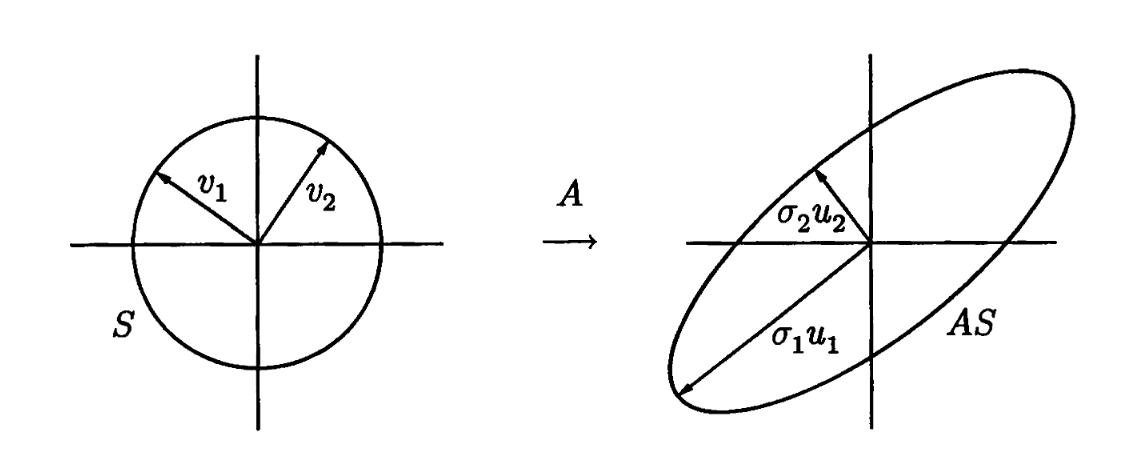
\includegraphics[scale=0.3]{images/Hyperplot.png}\\
    \caption{Fig 1. Représentation sous forme d'hyperellipses}
\end{center}
En écrivant cette égalité sous forme matricielle, nous obtenons:
\begin{align*}
	\left[
		\begin{array}{ccc}
			&&\\&&\\&A&\\&&\\&&
		\end{array}
	\right]
	\underbrace{
	\left[
		\begin{array}{c|c|c}
			&&\\&&\\v_1&...&v_n\\&&\\&&
		\end{array}
	\right]}_{V}
	=
	\underbrace{
	\left[
		\begin{array}{c|c|c}
			&&\\&&\\&&\\u_1&...&u_n\\&&\\&&\\&&
		\end{array}
	\right]}_{\hat{U}}
	\underbrace{
	\left[
		\begin{array}{ccc}
			\sigma_1&&\\&\ddots&\\&&\sigma_n
		\end{array}
	\right]}_{\hat{\Sigma}}
\end{align*}
En usant du fait que $V$ est unitaire, nous avons $A = \hat{U}\hat{\Sigma}V^*$. Ceci est la forme réduite, dans la forme complète $U$ a $m$ colonnes et $\Sigma$ $m$ lignes, mais c'est pratiquement équivalent à la forme réduite car les $m-n$ colonnes additionnelles de $U$ sont annulées par les $m-n$ lignes additionnelles nulles de $\Sigma$.\\\\
La décomposition SVD complète s'écrit donc:
\begin{align*}
	A = U \Sigma V^*
\end{align*}
où $A$ est une matrice $m\times n$ quelconque, $U$ est une matrice unitaire $m\times m$ contenant les vecteurs singuliers de gauche, $V$ est une matrice unitaire $n \times n$ contenant les vecteurs singuliers de droite, et $\Sigma$ est une matrice diagonale $m \times n$ contenant les valeurs singulières (toujours positives).\\
Cette décomposition existe pour toute matrice, mais n'est pas forcément unique.

\subsection*{Interprétation}
La SVD permet de mettre en évidence les composantes principales de la matrice $A$. En effet, en triant les valeurs singulières par ordre décroissant, nous pouvons observer les directions les plus accentuées par la matrice, et celles qui sont ignorées ($\sigma_i = 0 ~~ \forall i > rank(A)$). Ceci permet de résumer des données sans perdre beaucoup d'informations, en ne gardant par exemple que la moitié des valeurs singulières et les vecteurs correspondants.\\\\
$V$ et $U$ sont des matrices de changement de base.\\
Lorsqu'on applique $A$ à un vecteur $x \in \mathbb{C}^n$, nous pouvons décomposer la transformation en plusieurs étapes. D'abord, on lui applique $V^*$, changeant ainsi sa base de la base canonique vers les vecteurs $\{v_i\}$. Ensuite, chaque composantes est multipliée par la valeur singulière correspondante, et $m-n$ lignes nulle sont rajoutées, $x$ est donc maintenant représenté dans la base $\{u_i\}$. Pour finir, la matrice $U$ change la base vers la base canonique, ainsi si $x$ vaut par exemple $0.1v_1+0.9v_2$, alors $Ax$ vaudra $0.1\sigma_1u_1+0.9\sigma_2u_2$.\\
La SVD peut être vue comme une généralisation de la décomposition aux valeurs propres, la différence est que dans celle-ci l'espace d'entrée et de sortie sont les mêmes, or dans la SVD ça peut être des espaces de dimensions différentes.\\

\section*{Compression d'images}
La compression d'images consiste en réduction d'informations présentes dans le fichier afin de réduire sa taille, en réduisant le moins possible la clarté de l'image. Comprimer une image peut être pratique non seulement pour économiser de l'espace sur le disque dur, mais aussi pour réduire la quantité de bytes envoyés sur le réseaux par exemple.\\
Beaucoup de techniques de compression d'images existent, mais ici nous allons utiliser la SVD de manière assez intuitive pour grandement réduire la taille des images.

\subsection*{Utilisation de la SVD}
L'application de la SVD pour la compression d'images est assez basique. Chaque image peut-être représentée par une matrice tridimensionnelle $m \times n \times 3$, où $m$ est la hauteur en pixels, $n$ la largeur, et l'entrée $A_{ij}$ est un vecteur de taille 3 contenant les trois valeurs R, G et B, représentant avec un entier entre 0 et 255 les valeurs rouge, vert et bleu respectivement, pour le pixel $i, j$.\\\\
Afin de réduire la taille du fichier, nous aimerions réduire le rang des matrices superposées $R$, $G$ et $B$, car dans les formats d'images populaires comme png ou jpg, la redondance d'informations permet l'utilisation de techniques de compression propres aux formats.\\
Pour ce faire, nous divisons la grande matrice tridimensionnelle en trois matrices $R$, $G$, et $B$, ensuite, pour chaque matrice, nous appliquons la SVD, obtenant ainsi $U$, $\Sigma$ et $V$. Pour réduire le rang, nous sélectionnons les $k$ premières valeurs singulières et les vecteurs correspondants, on obtient donc trois nouvelles matrices $U' = U_{:,:k}$, $\Sigma' = \Sigma_{:k, :k}$, et $V' = V_{:, :k}$. Nous obtenons ensuite la matrice réduite $R(/G/B)_{red} = U'\Sigma'V'^*$.\\
Pour finir, on superpose les trois matrices réduites, et on les sauvegarde dans un fichier image du même format que le fichier d'entrée, réduisant ainsi la taille en gardant la même résolution. Il est clair que plus $k$ est grand, plus l'image est comprimée.

\subsection*{Résultats}
\begin{figure}
    \centering
    \hspace*{-3cm}
    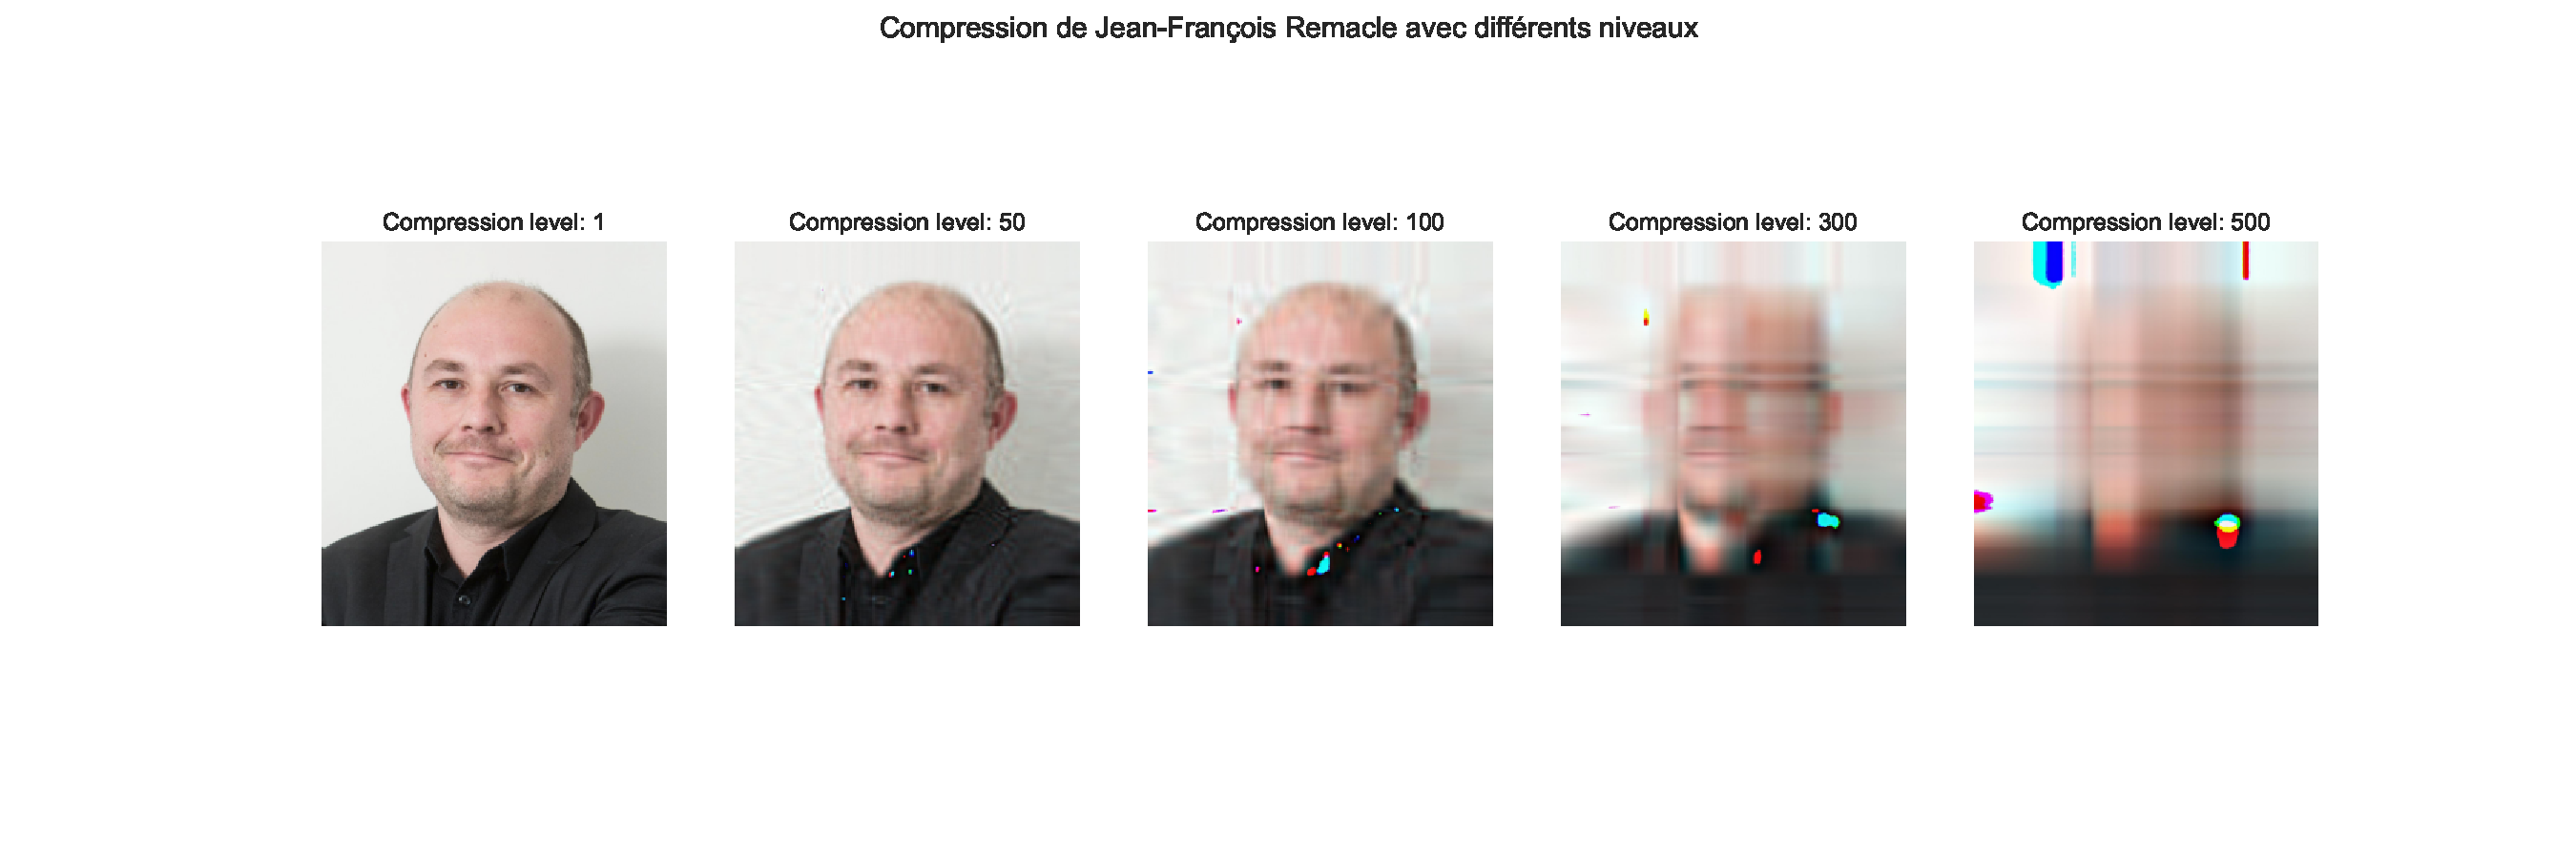
\includegraphics[width=1.3\textwidth]{images/compression_example.pdf}
    Fig 2. Compression de Jean-François Remacle avec différents niveaux de compression
    \label{fig:example}
\end{figure}
Quoi de mieux de tester notre algorithme qu'avec notre propre Lena: notre cher professeur Jean-François Remacle.\\
Nous pouvons constater que plus le niveau de compression\footnote{Ici, "niveau de compression" désigne le diviseur du nombre de valeurs singulières. Par exemple, si le niveau est de 2, alors le nombre de valeurs singulères (et donc le rang) est divisé par 2} est élevé, plus l'image est dégradée. Notons cependant qu'un niveau raisonnable de compression (e.g 50) conserve une qualité tout à fait raisonnable
\\\\
Nous pouvons observer que le ratio de taille sur une image aléatoire  ou choisie diminue fortement avec le niveau de compression. Il y a donc un compromis à trouver entre la conservation de la qualité et la compression. Un niveau de compression autour de 60-70 semble être un bon équilibre. À ce niveau, la taille d'une image est réduite de 10\% en conservant une qualité d'image tout à fait raisonnable.

\begin{minipage}[b]{0.49\textwidth}
    \centering
    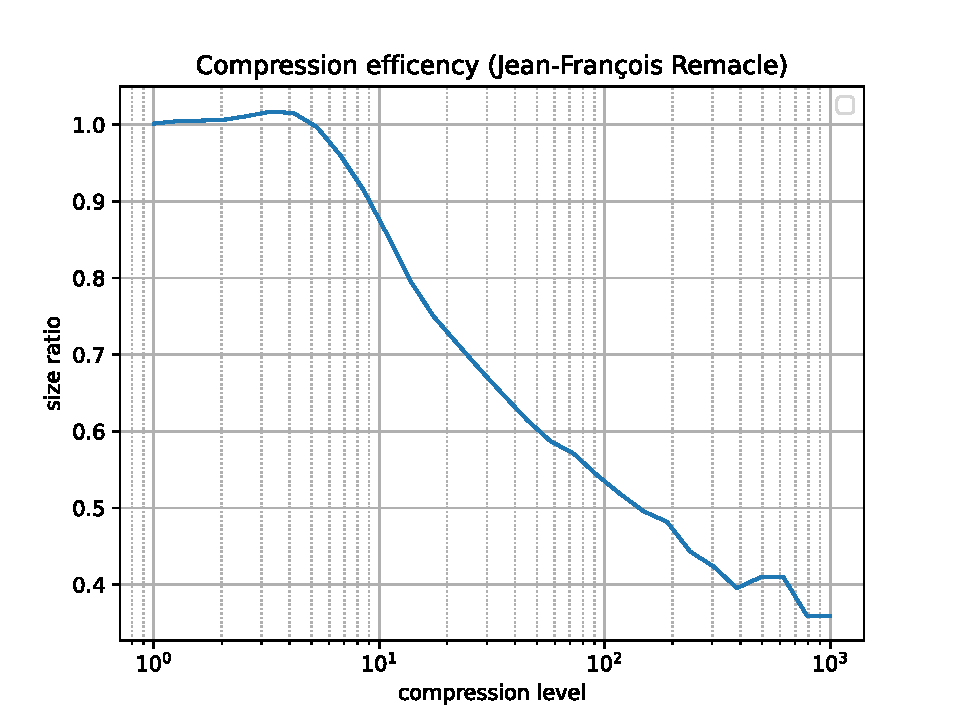
\includegraphics[width=1\textwidth]{images/Jean-Francois_Remacle_plot.pdf}
    \\
    \caption{Fig 3. Efficacité de compression sur une image choisie}
\end{minipage}
\begin{minipage}[b]{0.49\textwidth}
    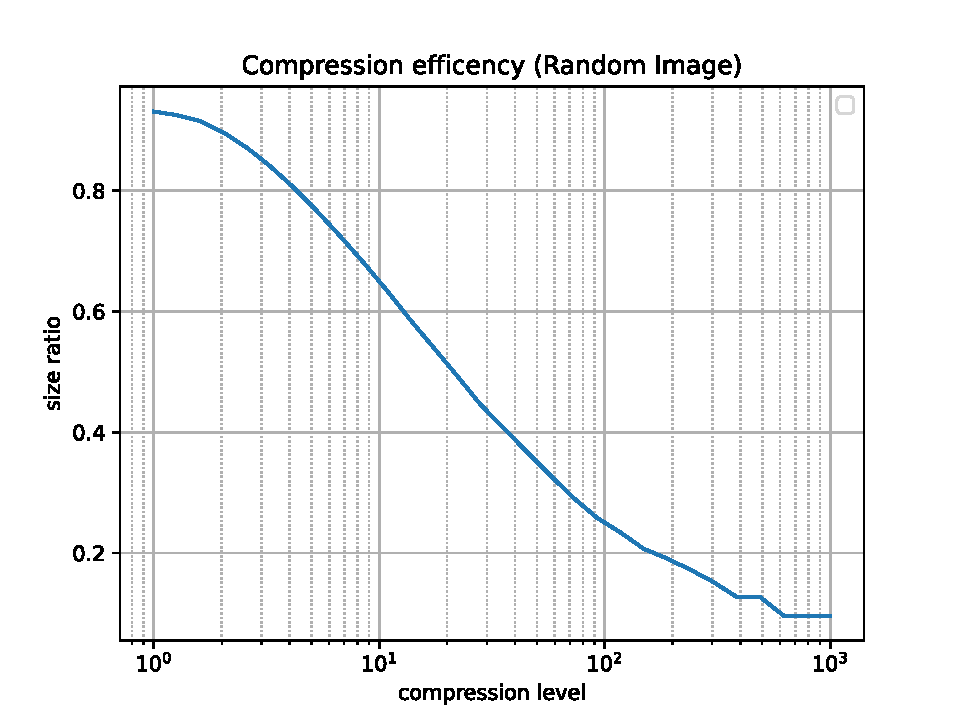
\includegraphics[width=1\textwidth]{images/Random_Image_plot.pdf}
    \\
    \caption{Fig 4. Efficacité de compression sur une image aléatoire}
\end{minipage}

\section*{Conclusion}
La SVD est une méthode élégante et générique qui trouve une application particulièrement à-propos dans le contexte de la compression d'image. 
Nous avons appliqué cette méthode sur les matrices R/G/B représentant les composantes couleur d'une image.
Pour de futurs travaux, il pourrait être intéressant d'envisager une parallélisation du traitement sur les trois canaux de couleur.

\begin{thebibliography}{9}
\bibitem{trefethen} L. N. Trefethen and D. Bau III, Numerical Linear Algebra. Philadelphia, PA: SIAM, 1997.

\end{thebibliography}

\section*{Annexes}
Nous avons réalisé une petite vidéo montrant Jean-François Remacle se faire progressivement comprimer.
\begin{figure}[H]
    \centering
    
\includegraphics[scale=0.1]{images/QR.png}
\end{figure}

\end{document}